\documentclass[12pt]{article}
	\usepackage[T1]{fontenc}
	\usepackage[utf8]{inputenc}
	\usepackage[british]{babel}
	\usepackage[a4paper]{geometry}
	\geometry{verbose,tmargin=3cm,bmargin=3cm,lmargin=2cm,rmargin=2cm,marginparwidth=70pt}
	\setcounter{secnumdepth}{3}
	\setcounter{tocdepth}{3}
	\setlength{\parindent}{4em}
	\setlength{\parskip}{1em}
	\renewcommand{\baselinestretch}{1.5}
	\usepackage{prettyref}
	\usepackage{textcomp}
	\usepackage{booktabs}
	\usepackage{lscape}
	\usepackage{setspace}
	\usepackage{indentfirst}
	\usepackage{fancyhdr}
	\usepackage{url}
	\usepackage[normalem]{ulem}
	\usepackage[table, fixpdftex]{xcolor}
	\usepackage{algpseudocode}
	\usepackage{bigstrut}
	\usepackage{enumitem}
	\usepackage{verbatim}
	\usepackage{mathtools}
	\usepackage{graphicx}
	\usepackage{longtable}
	\usepackage{chngpage}
	\usepackage{pdfpages}
	\usepackage{adjustbox}
	\usepackage[all]{nowidow}
	% package hyperref
    \usepackage[hidelinks]{hyperref}
  

	% biblatex
	\usepackage[style=authoryear,natbib=true,maxcitenames=2, maxbibnames=11,backend=biber,pagetracker=page,hyperref=true]{biblatex} \usepackage{csquotes}
	\renewcommand*{\bibsetup}{%
		\interlinepenalty=10000\relax % default is 5000
		\widowpenalty=10000\relax
		\clubpenalty=10000\relax
		\raggedbottom
		\frenchspacing
        \biburlsetup}
        
	% fixes the page number of the first page of each chapter
	\fancypagestyle{plain}{
			\fancyhead{}
			\renewcommand{\headrulewidth}{0pt}
			\renewcommand{\footrulewidth}{0pt}
			\fancyfoot[OC]{\begin{flushright}\thepage\end{flushright}}
    }
    
	% fancy headers for the thesis
	\fancyhead{}
	\fancyhead[RO]{\slshape \nouppercase \rightmark}
	\fancyfoot[OC]{\begin{flushright}\thepage\end{flushright}}
	\renewcommand{\headrulewidth}{0.4pt}
	\setlength{\headheight}{14pt}

	% add bibliography database
	\addbibresource{BA copy.bib}
	
	% space between biblio items
	\setlength\bibitemsep{1.7\itemsep} 
	
	% title without ""
	\DeclareFieldFormat[inbook]{title}{#1}
	% non-italic
	\DeclareFieldFormat[online]{tlaitle}{#1} 
	% title unquoted
	\DeclareFieldFormat[article]{title}{#1} 
	% no pp. 
	\DeclareFieldFormat[article]{pages}{#1} 
	% bold volume
	\DeclareFieldFormat*{volume}{\mkbibbold{#1}\setpunctfont{\textbf}}
	
	% no in:
	\renewbibmacro{in:}{} 
	
	% (volume)
	\renewbibmacro*{volume+number+eid}{%
			\printfield{volume}%
			%\setunit*{\adddot}% DELETED
			% \setunit*{\addnbspace}% NEW (optional); there's also \addnbthinspace
			\printfield{number}%
			% \setunit{\addcomma\space}%
			\printfield{eid}}
	\DeclareFieldFormat[article]{number}{\mkbibparens{#1}} 
	
	% edition.
	\DeclareFieldFormat{edition}%
	{(\ifinteger{#1}%
			{\mkbibordedition{#1}\addthinspace{}ed.}%
			{#1\isdot}).}
	
	% publisher and location p osition
	\renewbibmacro*{publisher+location+date}{%
			\printlist{publisher}%
			\setunit*{\addcomma\space}%
			\printlist{location}%
			\setunit*{\addcomma\space}%
			\usebibmacro{date}%
			\newunit}
	
	% shortauthor before author
	\renewbibmacro*{begentry}{%
			\ifkeyword{Key}{\sffamily}{}%
			\iffieldundef{shorthand}
			{}
			{\global\undef\bbx@lasthash
					\printfield{shorthand}%
					\addcolon\space}%
			\ifboolexpr{test {\usebibmacro{bbx:dashcheck}} or test {\ifnameundef{shortauthor}}}%
			{}%
			{\printnames{shortauthor}%
                    \addspace\textendash\space}}
                    
\title{Does the Financial Condition of Corporate Activist Investors Matter?}
\author{Leopold Ingenohl}


\begin{document}
\maketitle

\pagebreak


\section{Introduction}

\begin{center}
	Macht das überhaupt Sinn was ich schreibe? Kann man das nachvollziehen? 
\end{center}
% rethink sentence - not reporting requirements! 
Much attention has been recently given to the current Securities and Exchange Commission (SEC) reporting requirements for Schedule 13(D), governing the disclosure of beneficial ownership interests in excess of five percent of outstanding common stock of a U.S. public company \citep{Giglia2018}. Amongst other causes, it is due to significant gains for the subject's stock when the partial acquisition through a Schedule 13(D) filing is announced \citep{Akhigbe2007}. wer filed alles? 



% types of filer - bridge corporations
However, it is still largely unanswered where this upward drift comes from \citep{Greenwood2009}. An approach to this issue is objective of this thesis. Namely, analyzing the relation between the financial condition of corporate investors and the abnormal returns on the subject's stock and determining whether the financial condition has explanatory power for the latter. The following findings motivate this approach.  



In recent studies of what happens to the target's stock after such a filing, \citet{Collin-Dufresne2015} observe a positive significant market reaction to the subject's stock upon a more general sample of Schedule 13D filings 
	\footnote{The sample is only restricted on the subjects stock characteristics rather than on characteristics of the filers e.g. they exclude all filings which are not common stock (CRSP share code 10 or 11), whose prices are below \$1 and above \$1000 and which involve derivatives \citep{Collin-Dufresne2015}.}. 
\citet{Brav2008} have shown a favorable market reaction, 7\% - 8\% average abnormal returns in the (-20|20) event window, particularly to Schedule 13D's filed by hedge funds. Similar results have been shown by \citet{Klein2009} who observe 10.2\% average abnormal stock returns specifically for hedge fund targets.\\
In addition, \citet{Brigida2012} have shown an even higher runup if the acquirer is a private investor or a non-financial corporation. This is matching with \citet{Akhigbe2007} findings who observe greater gains for the target's stock if the partial position was initiated by a corporate bidder. Concluding, filings submitted by all investor types are followed by positive market reactions on the subject's stock but those submitted by corporations seem to have a stronger impact. This motivates the first hypothesis which assumes significant positive abnormal returns for Schedule 13(D)'s filed by corporations.
% Characteristics | Motivation | Reasoning - Why do they make minority acquisitions? 

Since the investing corporation is allowed to behave in an activist manner by filing a Schedule 13(D) 
	\footnote{In comparison the investor could file a Schedule 13(G) in which he would hold the shares passively hence with no intention to bring change.} 
\citep{Brigida2012} they can use their stakes to actively monitor and influence the target which is similar to the definition of an entrepreneurial activist by. 
	\footnote{\citet{Klein2009} define the entrepreneurial activist as an investor who buys a large stake in a publicly held corporation with the intention to bring change and thereby realize a profit on the investment.} \citet{Klein2009}
These stakes tend to be either made for the purpose of investment or far more importantly, as strategic investments \citep{Damodaran2005}, possibly resulting in business agreements, alliances or joint ventures \citep{Allen2000}. \\
% Topics: Acquisitions | Friendly Takeovers | Hostile Takeovers | Joint-Venture | Activism | Comparison | Comparison HF - Why do they behave activist? 
In a more direct approach however, these strategic investments can also help as a stepping stone towards full control \citep{Huang2017}. 
This approach is supported by \citet{Goldman2005} who find that mergers and takeovers are often preceded by the acquisition of a minority stake in the target. Whereas hedge funds use their stakes to change characteristics of the target (e.g. the board of directors or the strategic orientation) \citep{Klein2009} corporate filers are mainly focused on synergies in the form of strategic alliances or takeovers between them and the target. \citet{Akhigbe2007} observe that partial acquisitions, if carried out by corporate investors, are more likely to result in a full acquisition when compared to all other activist investors. This means that within the mass of Schedule 13D filings, institutional investors are unlikely to pursue a complete takeover whereas corporations are potential full acquirers \citep{Brigida2012}. The possibility of a takeover could be one explanation for the strong impact corporate filings have on the market, because the abnormal returns could be a reflection of investors' expectations of the target firms stock being acquired at a premium to the current price \citep{Goldman2005} especially with strong corporate bidders being likely to overpay in the event of a full takeover \citep{Akhigbe2007}.
These findings motivate the second hypotheses which assumes the highest abnormal returns occur in the event of a purpose of transaction statement involving a merger or a takeover of the subject.
%Objective: highlight the importance of the financial condition -- Background

However, in order to be able to bring change -- might it be in the form of a strategic alliance or eventually in a takeover -- the filing corporation should be in a condition of sufficient financial health. 
% insert the method of payments in a takeover 
A recent example on this matter is the public perception of the HNA Group. The financial condition of the HNA group, China's largest private conglomerate which over the past few years invested around \$US40 billion in businesses around the world, has currently been of great interest to financial news. Not least because they built up a 9.9\% stake of of around \$US4 billion in Deutsche Bank in 2017, which is just below the 10\% threshold above which stake purchases must be approved by Germany's financial watchdog but also because of their complex and nontransparent financing methods .
The financing of the group has come under strain as a result of an official crackdown on risky financing at acquisitive private enterprises in China. The highly leveraged group is now facing a potential cash-shortfall and liquidity issues resulting in a S\&P global rating downgrade referring to a a „deteriorating liquidity profile" of HNA. Although HNA group is  a private conglomerate, the financial condition of corporations seems to be of great importance to other market participants with that said, even in the context of minority acquisitions. Therefore, linking investors' financial condition to  underlying market reactions could be an explanation for the latter. This motivates the third and most important hypotheses, namely that abnormal returns, triggered by activist minority acquisitions, can be explained by the financial condition of the investor. 
% payment method in takeovers! 

% Topics: Abnormal Returns | Financial Condition | Activism | Hypothesis | Conclusion

Based on the previous findings of corporate activism, namely their strong impact on the subjects stock in the form of abnormal returns and future possibilities involving the target, the economic significance of corporations as filers of Schedule 13(D)'s seems to be apparent.

Yet in order to make these possible developments and expectations look credible -- amongst other things strategic alliances and takeovers -- the investing corporation somehow has to emit signs of sufficient financial strength. Therefore, the link between the financial condition of the investor and the subsequent abnormal returns on the target's stock is an interesting issue to examine. This in particular, is objective of the paper. What precisely are the effects of Schedule 13(D) filings by corporations on the subject's stock and can the financial condition of the corporation explain the market's reaction? Or in other words -- how important is the financial condition of the corporation behaving in an activist manner? 

The paper proceeds as follows. Section 2 reviews relevant literature on Schedule 13(D) filings, their effect on the market and the motivation behind corporate equity ownership. Section 3 describes the composition of the sample and identifies the corporate investor. Section 4 presents the market's response to Schedule 13(D) filings and Section 5 analyses the relation between target's abnormal returns and investor's financial condition.

\begin{comment}
	\section{Hypotheses}

\begin{enumerate}
	\item There are significant positive abnormal returns after the Schedule 13(D) filing of a corporation
	\item The purpose of the transaction has an effect on the market reaction 
	\item The financial condition of the investor can explain the market reaction
	\item The financial condition is most important, when the puspose of transaction invovles a future merger or takeover
	\item The financial condition looses its importance when the target is a poorly performing company and gains importance when the target is performing well 
	\item 
\end{enumerate}
\end{comment}


\section{Literature Review}

\subsection{Schedule 13(D) and Market Reactions -- Institutional Investors and Corporations}
%Topics: Historical Background | Information contained | Difference G and D

Section 13(d) of the Exchange Act of 1934 was passed in order to increase regulation of tender offers and accumulations of stock.
It acts as an early warning, signaling "every large, rapid aggregation or accumulation of securities, regardless of technique employed, which might represent a potential shift in corporate control" \citep[p.2]{Morrison2015}. 
This means that under Section 13(d), anyone who becomes the beneficial owner of 5\% of an issuer's equity securities registered under Section 12 of the Exchange Act must file with the SEC a Schedule 13(D) within 10 days after the acquisition. The filing informs shareholder about investors who could influence or change control of the issuing company \citep[p.110]{Giglia2016}. The investors filing such a Schedule 13(D) can be broadly classified into institutional investors (e.g. hedge funds or mututal funds), other entrepreneurial activists (e.g. individual investors) \citep[p.188]{Klein2009} and relevant for this thesis, corporate investors. Amongst others, the filing specifies the security and the issuer subject to the filing, the identity and background of the filer, and the purpose of the transaction.\\
Whereas filing a Schedule 13(D) allows the investor to behave in an active manner, a passive investor can equivalently file a Schedule 13(G). It is a short-form filing that can be utilized if an investor holds a beneficial ownership interest passively, with no intent to change control of the company \citep{Giglia2016}. So according to \citet[p.187]{Klein2009}, an entrepreneurial activist is as an investor "who buys a large stake in a publicly held corporation with the intention to bring about change and thereby realize a profit on the investment". Based on this approach, corporations filing a Schedule 13(D) confess to manage their investments actively, likewise confess to approach and interact with the target company and can therefore be called corporate activist investors. 
%Topics: Characteristics AR | Problems in Comparison | Motivation of HF | Activism

So far, there exist many studies that examine the effect the disclosure of such an activist investment has on the target's stock. With regards to short-horizon event studies, all these studies find positive and significant abnormal returns around the Schedule 13(D) filing date.\\ 
Dealing with investor activism, especially filings disclosed by hedge funds, \citet[p.1730]{Brav2008} find positive average abnormal returns in the range of 7\% to 8\% in the (-20,+20) event window. \citet[p.188]{Klein2009} have similar findings and observe 10.2\% average abnormal stock returns on the target's stock. In a more recent study on investor activism by \citet[p.410]{Denes2017}, the average valuation effect is evaluated to be around 5\%. A somehow different approach is found in a study of \citet[p.363]{Greenwood2009} who observe abnormal announcement returns of 2.36\% for a sample of activist portfolio investors and document that the ability to force the target into a takeover is the driving force behind the abnormal market reaction. Nevertheless, all studies observe positive abnormal returns around the filing date and results only differ in magnitude.\footnote{Comparing the the abnormal returns across studies can be misleading as the authors used different models and event windows for estimating the abnormal returns. \citet{Greenwood2009} use the market return model with matching portfolios and the CAR for aggregated abnormal returns; \citet{Brav2008} calculates the aggregated abnormal returns by subtracting the value-weighted market index from the buy-and-hold return; \citet{Klein2009} use a similar approach with buy-and-hold returns but make more adjustments.}

While all of these studies identify hedge fund activism, its motivation and the effect it has on the market, most of them leave filings submitted by corporations aside. \citet[p.29]{Brigida2012} however, note that if the acquirer is a non financial corporation abnormal returns in the (-10,-1) window are around 14\%. The reaction implies the market perceives such corporate investments as value generating for target. \citet[p.2803]{Allen2000} find abnormal returns of around 7\% in the (-10,10) period on corporate purchase announcements which are significantly larger if the announcement is accompanied by strategic investments. Their sample however is based on purchase announcements and therefore differs from studies on the effect of Schedule 13(D) filings.\footnote{In \citet[p.2801]{Allen2000} sample, the mean fraction of equity acquired in the sample is 14\%, and includes acquisitions of at least 5\% of voting shares only.} In addition \citet{Collin-Dufresne2015} find a positive significant market reaction upon a more general sample of Schedule 13(D) filings, including corporate investors but not explicitly addressing them.\\
So what is the motivation of corporations to engage in active equity ownership, thereby disclosing a Schedule 13(D), and why are these investments perceived as value generating?

% What is constrained, distressed? 
% Because financial distress possibly resulting in bankruptcy represents a state in which the firm cannot meet or has difficulty paying off its financial obligations to its creditors the reference to HNA Group made above is exemplary here as the group has problems in refinancing the enormously high debt burden. 



% Although the filing of a Schedule 13(D) can be seen as the trigger for the market reaction, the reason of why the abnormal returns occur is still largely unknown. However, \citet{Brav2008} find that if hedge funds engage actively, they have a high succession rate in achieving their main objectives. In a more recent paper conducted by \citet[p.12]{Brav2009} they list these objectives based on the sample of filings. The vast majority of these objectives focuses on general characteristics of the target and possible increase in shareholder value. They can be separated into five, not mutually exclusive, categories. The first objective is the believe of the hedge fund that he can help the manager maximize the shareholder value because they believe that the company is undervalued. The second includes activism that is based on the targeting firm's payout policy and capital structure. for the third objective, the hedge funds target issues related to business strategy, such as operational efficiency, mergers and acquisitions or growth strategies. The fourth objective is aimed at the sale of the target company with the majority to force a sale of the target company to a third party. The last objective includes activism targeting corporate governance. These motives are congruent with the \citet{Klein2009} definition of an entrepreneurial activist "who buys a large stake in a publicly held corporation with the intention to bring about change and thereby realize a profit on the investment". A more cautious definition is presented by \citet{Greenwood2009} who define an activist investor as someone who tries to change the status quo through voice, without a change in control of the firm. 

\subsection{Motives of Corporate Equity Ownership and Target's Value Increase}
% 13(D) = Minority Acquisition - Proxy 
%Topics: General Objectives | Definitions | Motivation | Minority Acquisitions | Toehold  

Corporate investments in other firms' equities can be be split into three broad categories. They can either be classified as ordinary, far more importantly as strategic and thirdly as stepping stones in a takeover process. 
In the sense of possibilities that might be reached, corporate ownership, in comparison to ownership by institutional investors, is unique \citep[p.2791]{Allen2000}.

\citet[p.1]{Huang2017} suggest that corporations make strategic minority acquisitions in other companies when they confront informational or integration barriers. 
Therefore, one reason for corporations to acquire a partial stake is that in the presence of alliances or joint ventures, minority acquisitions help to align the incentives of both firms involved and thereby decrease contracting and monitoring costs \citep[p.2792]{Allen2000}. This especially is of importance, if the strategic cooperation involves relationship specific assets and the investing corporation might be concerned with a holdup problem.\footnote{\citet[p.1023]{Ouimet2013} Defines the holdup problem as a decrease in the investors bargaining power in a renegotiation of the contract because the value of the initial investment is dependent on future cooperation with the target.} \citet[p. 2793]{Allen2000} show that in the years following a strategic investment,  targets increase investment expenditures, exhibit substantive gains in operating cash flow and the partial stake leads to significant benefits for both firms.\\
The second motive behind corporate minority investments is that if asymmetric information has an adverse effect on cost and availability of external capital for the target, the investment can provide capital directly to the issuing firm or validate its investment opportunities \citep[p. 2792]{Allen2000}. This is supported by \citet[P.1038]{Ouimet2013} who finds that the investment helps to overcome asymmetric information and thereby helps to certify the target for other outside investors.\\
Thirdly, by acquiring partial stakes corporations can effectively monitor or influence the target's management. When compared to institutional investors, a corporate investor has superior knowledge and operating expertise \citep[p.2792]{Allen2000} and can thereby further increase the target's operational performance.\\
But acquiring a minority position also helps to better assess real options, notably that of expanding. The acquisition of a minority stake helps to better assess the target for a potential majority acquisition \citep{Ouimet2013} and according to \citet[p.30]{Huang2017} gather more information before launching a bid for takeover. In this sense, by decreasing informational barriers the investments can help as a stepping stone towards full control \citep[p.3]{Huang2017}.\\
Because there exist two options two acquire full control of a publicly traded firm in the United States, either through a merger or through a tender offer \citep[p.2]{Offenberg2015}, \citet[p.1]{Betton2008} use the term takeover "for any acquisition of corporate control through the purchase of the voting stock of the target firm, regardless of whether the bid is in the form of a merger agreement or a tender offer".\\
For merger agreements, a beneficial ownership of a partial stake helps to speed up the shareholder approvement process, induce the acquirer to fully commit to the merger and therefore increases the probability of a successful takeover \citep[p.19]{Betton2008}.
Prior to the takeover bid, the corporations can also acquire a toehold where neither management nor target's shareholders know of the investor's takeover intention until the announcement of a Schedule 13(D) is due. Following \citet[p.158]{Eckbo2009} acquiring a toehold, before initiating the takeover bid, is compelling. It reduces the number of shares that must be bought at the full takeover premium and it can be sold at a profit if a rival bidder wins the target.\\
\begin{center}
	what is the gain on the target's stock?
\end{center} 
Concluding, corporations filing a Schedule 13(D) and thereby confessing to actively manage the investment have several reasons to do so. However, overcoming informational and integration barriers seems to pervade in almost all cases. Strategic investments generate value, financing validates investments opportunities and help to overcome information asymmetry and partial stakes in the process for full takeover bring value. Therefore, the information contained in corporate Schedule 13(D) filings is valuable. 
\begin{center}
	Value of SC 13(D), still largely unanswered where the announcement premium comes from \citep[p.363]{Greenwood2009}
\end{center}

But beyond the motives of corporations to actively engage in another firm and the benefits such an investment brings to both, to what extent does the corporations financial condition matter when the market values such activist investments?  One could assume that a financially strong investor proxies for the investment's value creation and therefore should have an impact on the market's assessment of the present and future value of the target. Determining questions would be whether the investing corporation is able to establish a profitable collaboration, whether it is able to bring value to the target, whether it can ensure assertiveness in a takeover or whether it is likely to pay a large premium in the event of a takeover. At large, does the financial condition of corporate activist investors matter when the market's reacts to Schedule 13(D) filings?\\
Under the assumption of perfect capital markets, the financial structure of the investor should be irrelevant to investment and the markets valuation of it, because "external funds provide a perfect substitute for internal capital" \citep[p. 141]{Fazzari2016}. This however, is not the case for financially constrained firms because they face an inelastic supply of external capital \citep[p.1]{Farre-mensa2013}. Consequently, firms who are able to raise substantial amounts of external capital without much of an increase in the cost of capital are considered as unconstrained \citep[p.1]{Farre-mensa2013}. Therefore if a firm is constrained, likewise faces a cost disadvantage of external finance, the investment would be driven by fluctuations in the cash flow \citep[p. 142]{Fazzari1988} . This in turn would imply a different investment behavior of constrained firms when compared to healthy firms. \\
\citet[p.450]{Bhagat2005} investigate whether the same can be assumed about the investment policy of distressed firms and find it does. They also show that firms in distress invest less and "behave differently from financially constrained firms" \citep[p.461]{Bhagat2005}. 
In addition, the size of the investing corporation could also play an important role in the market's investment valuation of the investment in the target. Large firms may enjoy easier access to capital markets, receive higher credit ratings for their debt issues and pay lower interest rates on borrowed funds \citep{Saquido2003}

% Considering the takeover process mentioned above, the necessity to file a Schedule 13(D) and thereby confirm the beneficial ownership of at least 5\% of the outstanding stock, prior or while negotiating the takeover bid, is more difficult to comprehend. Nevertheless the success of a potential takeover seems to be especially dependent on the bidders condition to be faster and stronger than potential competitors, the initial bidder has to ensure assertiveness. In order to appear strong (the market perceives the acquirer as a winner) the acquiring company must have sufficient financial strength. In the first place to make the takeover process credible to outside investors and secondly to signal the ability to pay the takeover premium. In any case, the target's outstanding shares have to be acquired at a premium to the price prevailing at the filing date either trough cash, stock or a mix of both. Besides that, a strong acquirer could have more bargaining power in persuading the target's shareholders to approve the merger and successfully carry out the takeover. 
% To faciliatate thhareholders of the target might sign a voting agreement in favor of the acquirer in which they agree to vote the shares in a way expressed by the acquirer - corporations might have to sign a Schedule 13(D) although they did not buy the shares but have their voting power.
% Whereas a merger agreement is the result of negotiations between the investor and the target's management, in a tender offer the acquirer makes a direct bid to target shareholders to purchase the target shares.
% By negotiating with the target's management a merger agreement might appear as the safer option. However, it does not lock up the target from potential competition because the director fiduciary duties require the target board to evaluate competing offers until the agreement is approved by the shareholders \citep{Mitchell2011}.  To prohibit the acquirer of purchasing target shares in the market during negotiations, parties often sign a standstill agreement \citep{Mitchell2011}.  
% Another possibility is the purchase of ownership in the target prior to the start of the takeover bid - a toehold. Neither management nor target's shareholders know of the acquirers takeover intention. Following \citet[p.158]{Eckbo2009} acquiring a toehold, before initiating the takeover bid, is compelling. It reduces the number of shares that must be bought at the full takeover premium and it can be sold at a profit if a rival bidder winds the target but it can also create hostility with the target's management \citep{Goldman2005}. This is the reason why toeholds are much more common in hostile bids \citep{Mitchell2011}. On the other hand \citet[p. 216]{Povel2014} suggest that toeholds are not much different to the general minority acquisitions. Because the toeholder might negotiate the right to nominate one or more directors in the target's board, they open the door to a more intensive cooperation. According to \citep{Mitchell2011} bidders initiating a takeover bid in the U.S. over the period 1980-2005 offered all cash as payment in 26\% of the cases, all stock in 37\%, and a mix of both in 37\%.
\section{Data -- Constructing the Sample}

The data that is used to analyse the relation between the investor's financial condition and the market reaction to Schedule 13(D) filings,  is primarily composed of information contained in the filings from SEC's Edgar database and secondly of data on stock and fundamentals,  accessed through Wharton Research Data Services (WRDS). The sample of Schedule 13(D) filings is consctructed as follows. First, using an automated search script, 48'626 filings from the 20 year period starting in January 1996 and ending in December 2016 were identified.  The script identifies all Schedule 13(D) filings that appear on EDGAR and extracts the following information: name of filer and subject, the CUSIP of the underlying security and the filing date. Next, to only have filings submitted by corporations hence to separate corporate investors from institutional investors (i.e. hedge-funds or pension-funds), 10-K reports were cross-referenced with the initial sample of filings.\footnote{10-K reports were used to identify corporations because "managers of publicly traded firms are required to produce public documents that provide a comprehensive review of the firm’s business operations and financial condition and an important financial disclosure document created by managers to communicate with investors and analysts is the annual report filed pursuant to the Securities Exchange Act of 1934 the Form 10-K." \citep[p. 1643]{Loughran2014}} To be considered, the filer had to have a 10-K report submitted at least 12 months prior to the filing which reduced the sample to 3'325 filings. As daily stock returns and prices for the target's securities come from the Center for Research in Security Prices (CRSP) the subject not only had to have SEC's Cusip identifier but also an active link between Cusip and CRSP's Permno identifier. For estimating the market reaction to Schedule 13(D) filings, there had to be sufficient stock data for the remaining 1'467 filings. The data was only available to subject of 1'151 filings. 
The accounting fundamentals for identifying the investing corporation's financial condition were extracted from the Compustat database. To be included, the filer had to have a valid link between its 10K-CIK and Compustats's Gvkey indentifier. This further reduced the sample to 1'014 filings. In the next step and based on Fama \& French's 48 industry classification, all filers belonging to the trading industry (industry code 47) were excluded. This was done for the reason that the investment behavior of corporations in this industry differs substantially from that of other industries. This left a sample 898 filings for which data on specific financials was only available for 644 investors. From the remaining 644 filings, the purpose of the transaction was manually extracted. During this process, Schedule 13(D/A) filings (amendments to previous filings) that were mistakenly classified as original Schedule 13(D) filings and filings not submitted by corporations were excluded. This reduced the final sample to 494 filings.\footnote{The only exception were filings submitted by the Commerce Group Inc., which provides both insurance and, real estate, brokerage services. These filings were excluded because (1) the largest part of them were amendments, (2) the amount of filings submitted was disproportionately and (3) all purposes of the transaction were general investments in an investment fund.} 

\subsection{Measures of Financial Condition}
As the investors financial condition is hidden in its statements and there exists no such line specifically noting whether the investor is ought to be in a good or bad condition, several determining measures are established. By allowing to separate the original sample into different sub sample based on the financial condition, these measures make the condition of different corporations comparable. A detailed listing of each scores components and calculation can be found in Appendix A.\\
\citeauthor{Piotroski2000}'s (\citeyear{Piotroski2000}) F-Score is used to proxy for investors general strength. This is done for the reason that it is a "... composite measure of firm strength" \citep[p. 496]{Fama2006} and secondly considers in what directions the fundamentals of a company are trending and whether general health conditions are met \citep[p.5]{Mohr2012}.\footnote{In order to legitimize the explanatory power of the F-score in separating strong from weak firms Piotroski formed portfolios consisting of value firms. In doing so, he showed that an investment strategy of shorting expected losers (weak firms) and buying expected winners (strong firms) would "generate a 23\% average annual return" \citep[p. 4]{Piotroski2000}. This is matching with \citet{Hyde2014} results, who observe significant return premiums for stocks with a high F-score over stocks with a low F-score.} Although \citet[p.6]{Piotroski2000} established it to separate strong from weak value firms \citet[p.16]{Mohr2012} shows that its application on growth stocks yields similar results.\footnote{This is in line with \citet{Piotroski2000} and confirms earlier research conducted by him.} The score consists of nine binary signals from fundamental analysis that result in a final score ranging from zero to nine, with nine being the best outcome. As its broad application on stocks is possible and because it is based on fundamental analysis, using it to separate the sample into strong and weak investors seems promising.  
Although corporations might have a score in the lower region, this per so does not say the corporation is weak. For simplicity however, firms within the range of (0-3) points are labeled as weak and those with a score ranging between (7-9) as strong. This marking is different to \citeauthor{Piotroski2000}'s (\citeyear{Piotroski2000}) original application but it yields two larger sub-samples which at the same time are more independent from rare outliers \citep[p.12]{Mohr2012}.

The Whited-Wu index according to \citet[p.543]{Whited2006} and with reference to \citet[p.38]{Farre-mensa2013} is applied to delimit the corporations that might be financially constrained. Following convention, firms are sorted into terciles based on their index value. Frims in the top tercile are coded as unconstrained whereas firms in the bottom tercile are coded as constrained. The Kaplanz-Zingales index also identifies financially constrained firms, but \citet[p.]{Farre-mensa2013} note that it appears to be more of an outlier. 
\begin{center}
	add more arguments why not kz index! 
\end{center}
Although \citet{Khatami2014} note that more recent literature has questioned the reliability of constraint measures, the Whited-Wu index  blabla. To control for possible misclassification, corporations are also classified according to their credit rating. Therefore, firms without a S\&P 500 domestic long term issuer credit rating are treated as constrained \citep[p.6]{Farre-mensa2013} which again yields two sub samples. 

To further enrich the analysis, \citeauthor{Altman1968}'s (\citeyear{Altman1968}) Z-score identifies corporations in financial distress. The score is a fundamental indicator that according to \citet[p.5]{Mohr2012} shows statistically significant results in predicting the bankruptcy of a company and has become a popular and widely accepted measure of financial distress \citep[p.2903]{Campbell2008}. 
With regards to the above the Z-score is a prediction of corporate bankruptcy \citep[p.594]{Altman} and is computed with a predefined model that considers five variables ratios of financial analysis. With respect to a threshold of 2.675 \citep[p.607]{Altman1968} the final score is put into perspective, according to which firms below can be classified as firms in bankruptcy and those above as in non-bankruptcy. 

With regards to the upcoming analysis, firms are classified as being in a good (bad) financial condition when they either belong to sample of strong (weak) firms, to the samples of undistressed (distressed) firms or to the sample of unconstrained (constrained) firms.


\subsection{Descriptive Data}

Table 1 identifies the sample's Schedule 13(D) filings based on several criteria. Column (1) presents information on all filings. In a first subdivision of the investors, Column (2) and (3) give information about filings submitted by investors categorized according to Piotroski's F-Score.
Panel A shows that the total sample consists of 498 filings, with 109 submitted by strong and 83 by weak investors. The imbalance in filings for the two groups is due to the F-score's unequal distribution across investors. 
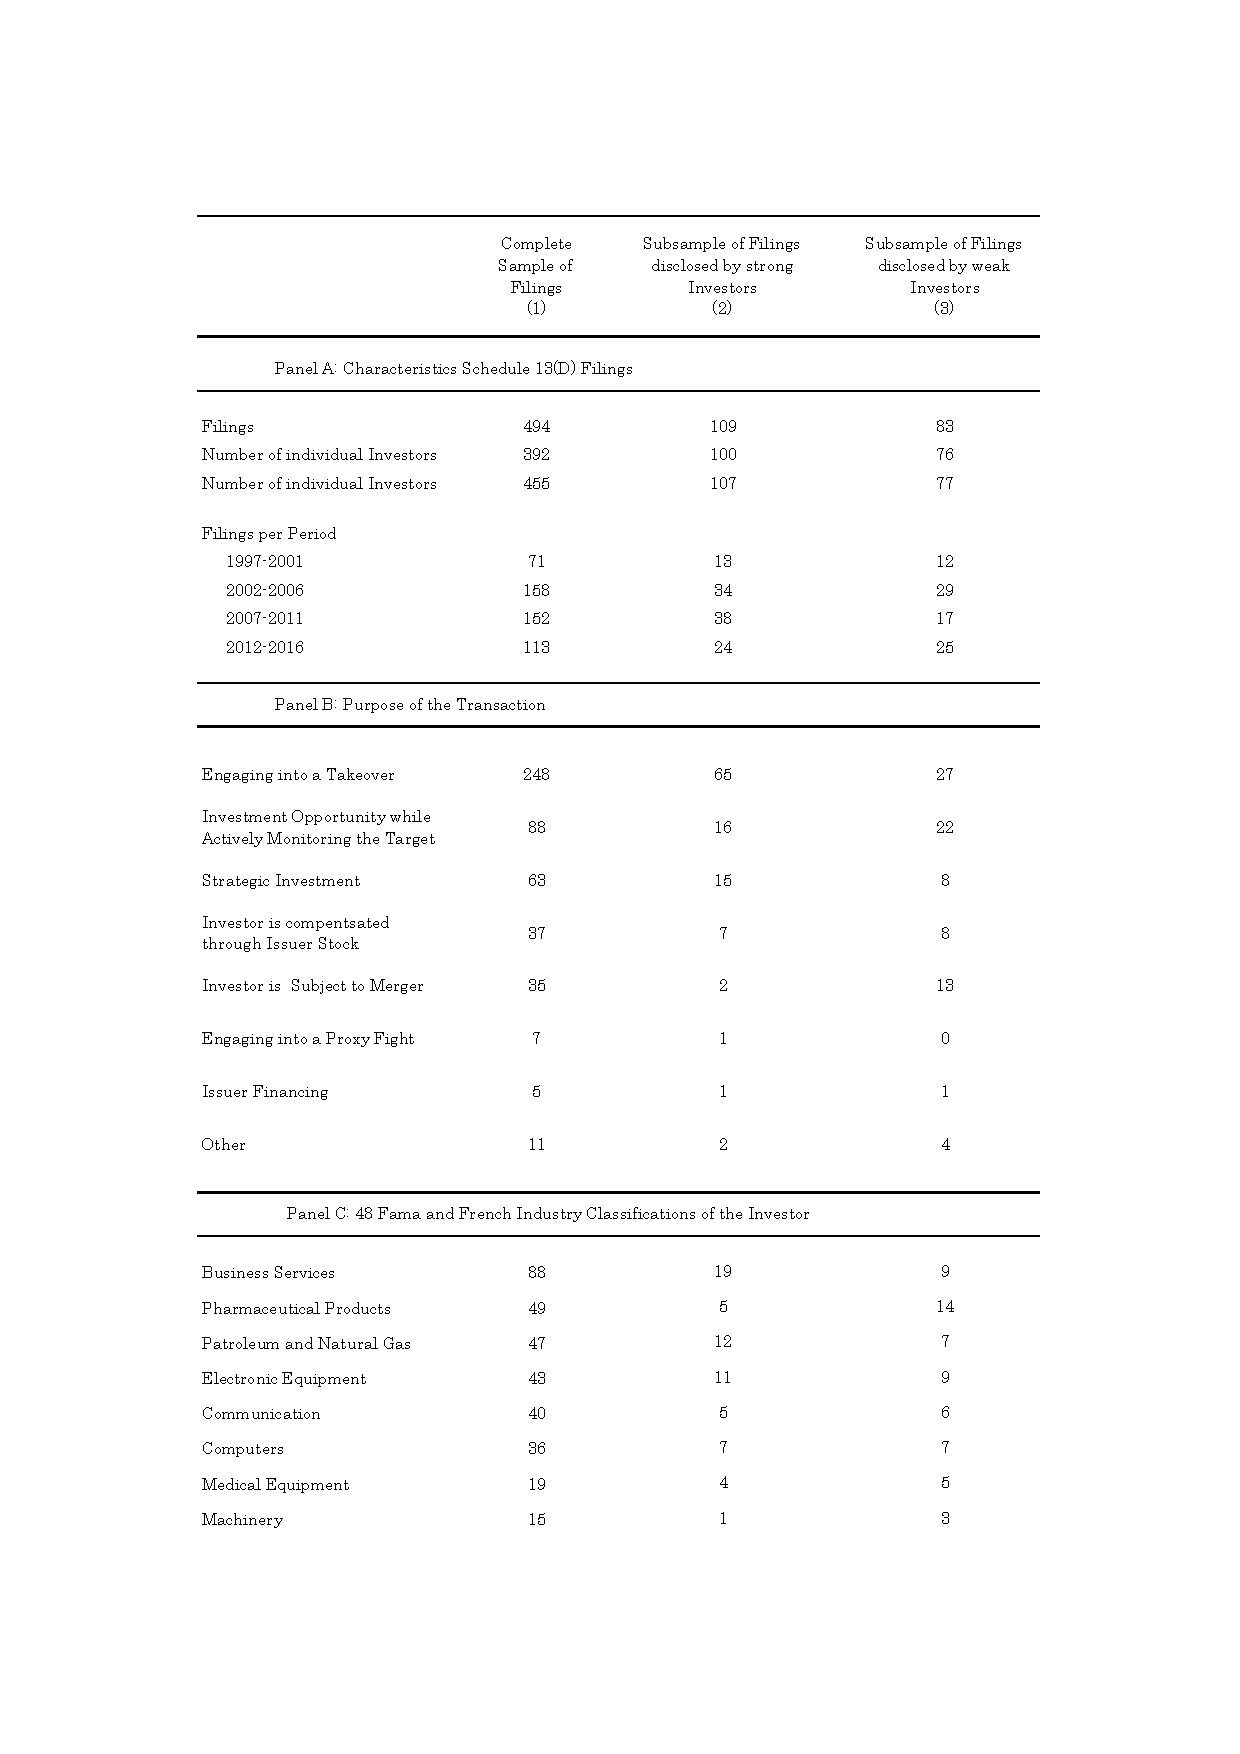
\includepdf[pages={1},pagecommand={}]{Descriptive_Statistics_copy.pdf}
The filings were submitted by 392 individual investors but 455 individual firms were subject to filings. This means that occasionally either one firm was investing in multiple targets (e.g. 6 filings submitted by AT\&T) or a target was subject to more than one filing (e.g. four filings for investments in Clearwire Inc.). Across the sample, multiple occurrences are not common.\\
The smallest amount of filings in the sample were disclosed in the 5-year period of 1997-2001. In the following ten years however, more than 60\% of the sample filings were submitted. The largest amount of filings was in the 5-year prior to the financial crisis. It is noticeable that the number of filings in the years around the financial crisis is higher than the number of filings reported for the span of 2012-2016. An explanation could be the merger wave of 2007 \citep[p.19]{Huang2017} which lead to an increase of Schedule 13(D) disclosures. Also noticeable is that one quarter of the filings from this period were submitted by strong and only around 10\% by weak corporations.


Panel B lists the extracted "Purpose of Transaction", which represents item 4 in Schedule 13(D) filings. The purpose is only explicitly stated if it occurred in at least five filings. Additionally, the purpose "engaging into a takeover" and "strategic investment" represent several purposes. According to \citet[p.1]{Betton2008}, filings disclosed with the purpose of a merger agreement, tender offer or hostile bid are grouped under the purpose "engaging into a takeover"  and filings due to alliance agreements, license agreements, strategic acquisitions and joint ventures are grouped under the purpose "strategic investment". A detailed description on how the filings were categorized can be found in Appendix B. 
Remarkable is the fact that around half of the stock acquisitions were made in the course of engaging into a takeover process. This is interesting as for around 50\% of the filings, the investor's financial condition should be a part of the market's target stock valuation. More than double the amount of these filings were submitted by strong corporations.\\
On the other hand, this ratio switches for filings in which the investor is subject to a merger -- the target's shares were acquired to distribute them to own shareholders as a form of payment.\\
With 88 filings, the second most reported purpose due to which the Schedule 13(D) were disclosed is because the target is considered to be a good investment opportunity while the corporation wants to actively monitor the investment. In the bottom line these filings do not directly imply future collaboration between the two firms.\\
Following actively held investments, strategic investments are the third largest group of purposes due to which the filing was disclosed. Different to the former, they are based on the premise of future collaboration between investor and target. Although potentially of high interest, they represent only 10\% of filings. Only 7 filings were submitted due to a proxy fight only 5 reported the investment's purpose was to finance the issuer.\\
These findings support the evidence on why corporation would actively hold equity ownership, while a majority of the filings are disclosed due to takeover activity or strategic investments.
According to Fama \& French's 48 industry classification code, panel C presents the major industries to which the investors belong to. Shown are only industries, in which at least 15 investing corporations operate. For the complete sample of investors, 42 out of the maximum 48 industries are represented. As mentioned previously, the sample is restricted by excluding the trading industry due the irregular investment behavior. The highest industry representation is that of business services with 88 filings, followed by the industries of pharmaceutical products and patroleum and natural gas.
	\begin{center}
		a lot of investments typical in those industries? 
	\end{center}
\begin{comment}
	\subsection{Examples of Corporate Activism}
	In this subsection, two cases of corporate investments into other firms are being described. The first example is takeover the second is strategic investment. 

	\subsubsection{Pfizer Inc. and Icagen Inc. }
	On June 24, 2011 Pfizer filed a Schedule 13(D) in which it declared an ownership of 14.2\% in Icagen Inc.. Pfizer was initially engaging with Icagen in accordance to a "collaboration agreement" dated August 13, 2007. In the purpose statement of June 24, 2011 Pfizer wrote: 
	\begin{center}
		"Pfizer is evaluating the possibility of entering into a strategic transaction with Icagen, which could have the effect of influencing or changing the control of Icagen by means of stock or asset acquisition or merger"
	\end{center}
	Consequently, the filing can be considered as firms strategic investment and the purpose statement can be classified as indicating that Pfizer wants to further strategically invest in Icagen.
	The ownership of 14.2\% in Icagen was acquired between 2007 and 2008. The collaboration agreement on August 13, 2007 involved the "discovery, development, manufacture \& commercialization of pharmaceutical compounds and products that modulate three specific sodium ion channels as potential new treatments for pain and related disorders". The investment resulted in Pfizer appointing the treasurer and president of Icagen as their proxies. 
	In order to extend the collaboration agreement, on September 17 2009 Pfizer and Icagen entered into the first amendment to the agreement. 
	On September 21, 2010, one year later, they entered into a second amendment to the collaboration agreement which would extend it until December 31, 2011. In the course of a further collaboration between Pfizer and Icagen after the expiration of the collaboration agreement , Pfizer filed this Schedule as stated in the purpose statement above.
	\pagebreak	
\end{comment}

\section{Identifying the Investors prior to the Schedule 13(D) Filing and Measures of Financial Condition}

After being familiar with general characteristics of the sample's filings, this section focuses on identifying the corporations prior to their Schedule 13(D) filing.
Table 2 introduces the four different measures of financial condition. For each measure there exist two sub-samples. By the virtue of each measure, the two samples do not necessarily have to add up to the total number of filings. Hence for the $F$-score, separating weak from strong investors yields a sample of 109 strong and 83 weak firms. Applying the $Z$-score to the sample, 103 investors are identified as distressed and 351 as undistressed and according to the terciles from the Whited-Wu index, 164 investors are financially constrained and 165 are not. Only for the S\&P credit rating do the two samples include all corporations with 238 firms missing a credit rating and 256 having one. This means, there exist a total of eight sub-samples plus the initial one.\\
For each sub-sample, table 2 reports the mean [median] of several key financials. For the complete sample standard deviation and both, lowest and highest value are shown additionally. All reported data corresponds to the investor's fiscal year which is closest to the filing date and the reported values are winsorized at the 1\% and 99\% levels so that extreme values are replaced by the respective percentiles. This enables a presentation of more meaningful mean statistics \citep[p.203]{Klein2009}. For simplicity, firms categorized as weak, distressed, constrained or missing a credit rating are forthcoming considered to be in a unfavorable state whereas their counterparts are to be in a favorable state. % For all following tests, the $t$-statistics are for difference in means, assuming unequal variances between the samples. The $Z$-statistic is a Mann-Whitney rank-sum test for equality of medians on unmatched data and 

Panel A reports two ratios on profitability. The first one is returns on assets (ROA), defined as earnings before interest and taxes (EBITDA) to total assets and the second is the ratio of cash flow from operations to total assets. 
For all measures, those identified to be in the unfavorable state have a ROA which is significantly lower when compared to their counterparts. Furthermore, the average ROA for weak and distressed companies is negative meaning they made a loss in the fiscal year prior to the filing. Accordingly, their average cash flow is negative as well although now constrained firms have a negative value as well. his could have further implications as \citet{Bhagat2005} note that distressed firms have a negative cash-flow sensitifity and thereby invest more when cash is low. Again, the difference among the corresponding sub-samples is apparent across all measures.\\
Panel B reports ratios on cash balances and debt. Firms considered as weak and constrained and those missing a credit rating have higher cash and short-term investments compared to their counterparts. Only distressed firms have a lower ratio due to their very nature of having issues refinancing their debt. Constrained firms have the highest ratio with around 33\% of the total asset value in cash and short-term investments. Similar, they and firms without a rating have considerably more cash when compared to their counter samples, reflecting their dependency on internal funds when it comes to investments \citep{arg}. With regards to weak and distressed firms, the difference in the cash to asset ratios are marginal. 
Book leverage, defined as long-term debt plus current debt to total assets \citep[p.1440]{MacKay2005} is unsurprisingly the highest for distressed firms as it is one of the reasons they are considered distressed. 
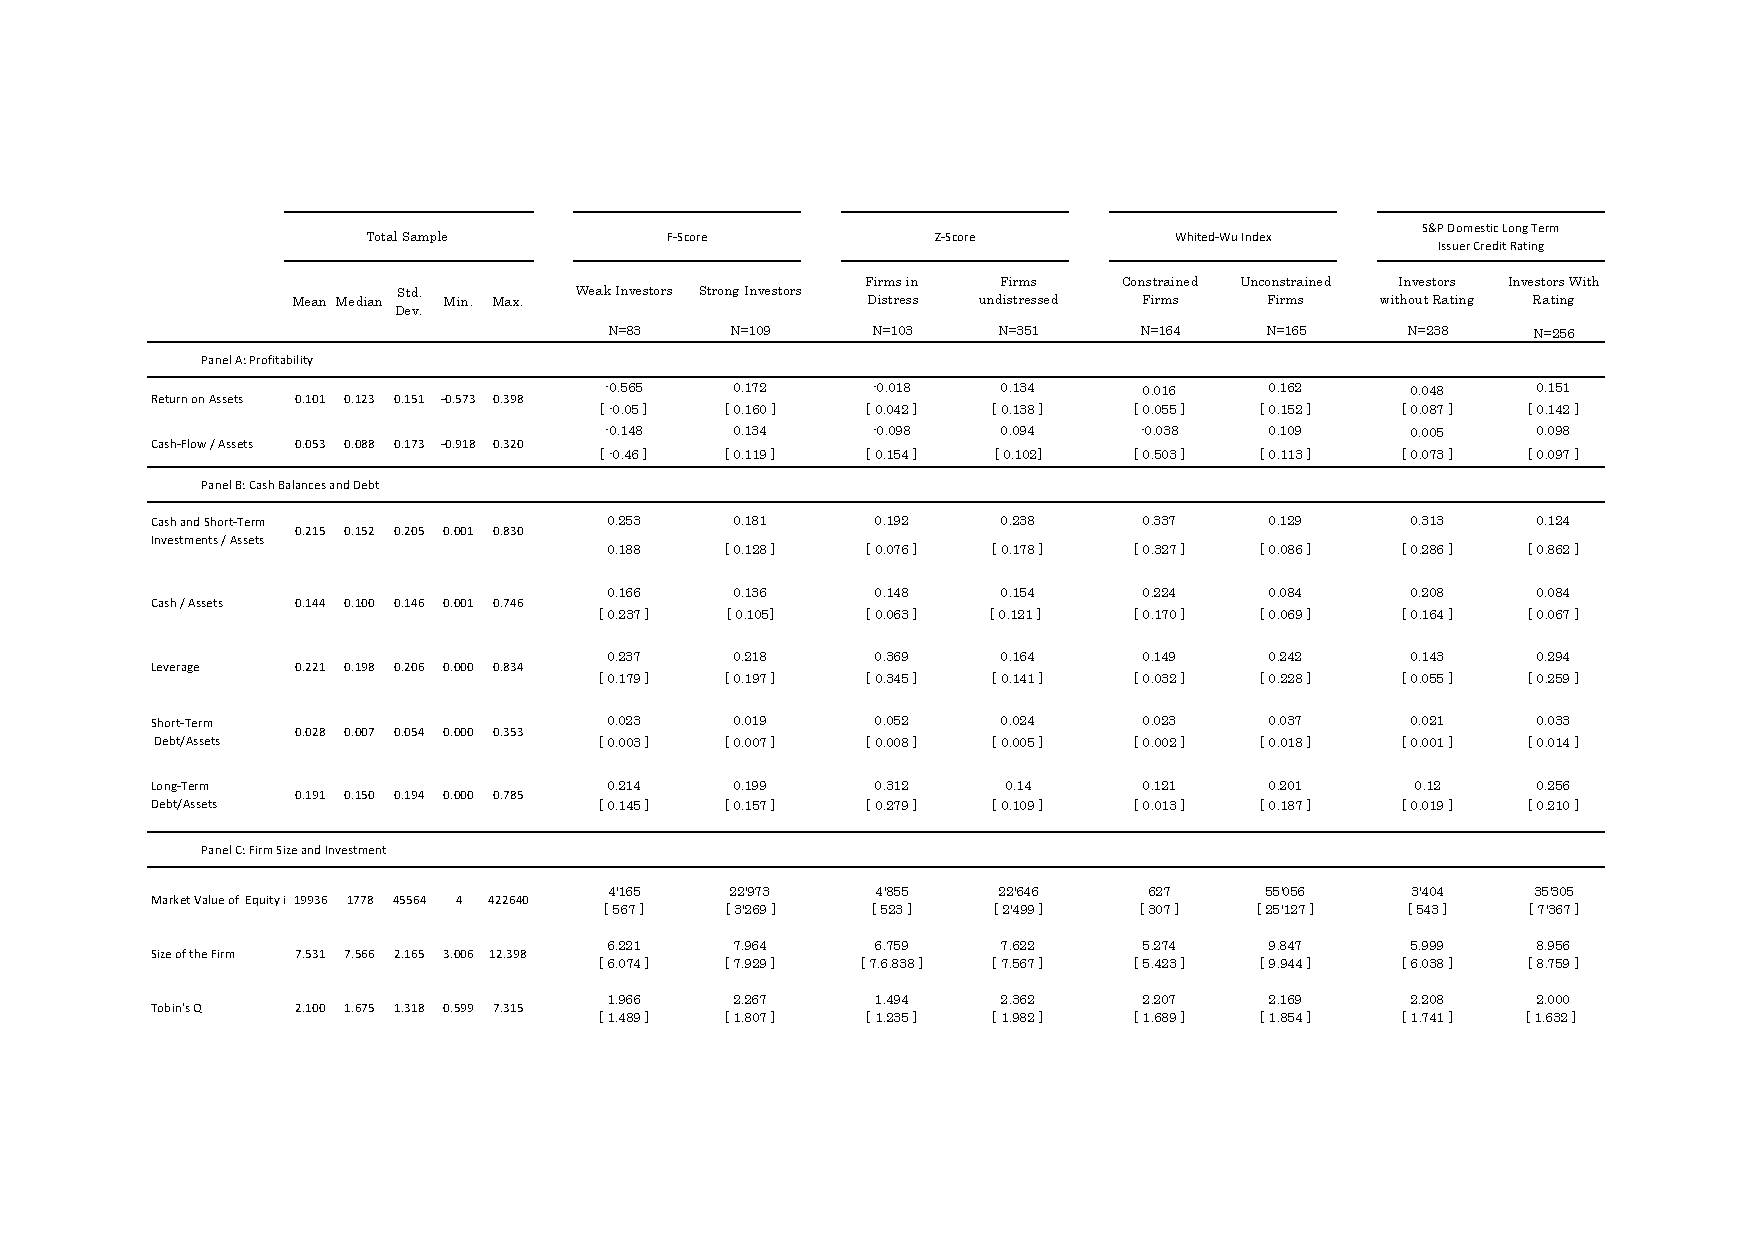
\includepdf[angle={90},pages={1},pagecommand={}]{Summary_Statistics_copy.pdf}
Weak and strong firms have a similar leverage whereas firms without a credit rating or constrained ones have higher leverage compared to the counter sample. Across all measures, the ratio of short-term debt to total assets is fairly small and only marginal differences among the sub-samples exist. 
Reflected in the companies leverage, long-term debt is the highest for distressed firms and unconstrained firms and those with a rating have a considerably higher long-term debt to asset ratio. This is comprehensible, as they have better access to external financing.\\
As Panel C reports financials on firm size and investment, all companies considered to be in the unfavorable state have a market value of equity significantly lower. The largest difference is among constrained and unconstrained firms. Similar differences are apparent in the size of the firms, defined as the natural logarithm of total assets. This suggests that size is an important determinant across all measures and independent of the measures. Lastly, Panel C presents Tobin's Q which proxies for investment opportunity \citep[p.1441]{MacKay2005} and is computed according to \citet[p.1]{Khatami2014}. Constrained firms, likewise those without a rating have a higher Tobin's Q which may be due to their unexploited investment opportunities \citep{Whited2006}

Concluding, firms in the unfavorable sub-samples are considerably smaller in size, less return on assets and small cash-flow and tend to have more cash. Compared to their counter-sample, constrained firms and those without a credit rating have less debt but higher values of Tobin's Q.


\section{Market Returns to Initial 13(D) Filings -- Abnormal Stock Returns}
% Intention
As this thesis seeks to analyze whether the financial condition of the activist corporate investor matter, abnormal share price reactions around the filing date identify the effect the 13(D) filing has on the target's stock, after accounting for general market movements.
The set up of the event study performed for this purpose is as follows: The time line consists successively of the estimation window, in which parameter estimates are obtained, the event window for which the abnormal returns are computed and the post event window. 
The filing date, as reported by the SEC and reported on EDGAR is set as the event day. For simplicity, the event window [x,y] is determined relative to the event day 0 with x days before and y days after the filing date. Abnormal returns are computed for various event windows. For that reason, the estimation window is set 120 days prior to the largest event window. With the largest event window starting 30 days before the event day, the estimation window begins 150 days prior to the actual event day.\\
The abnormal return $AR_{i,t}$ for the target's security $i$ at day $t$ is defined as the difference between the actual (observed) return $R_{i,t}$ and the expected return $E(R_{i,t}|X{t})$ given the absence of the event \citep[p.15]{MacKinlay1997}:
	\begin{equation}\label{eq:1}
		AR_{i,t}=R_{i,t}-E(R_{i,t}|X_{t})
	\end{equation}
The expected return $E(R_{i,t}|X{t})$ is the result of an estimation based the market model, in which the value-weighted NYSE/Amex/Nasdaq index from CRSP proxies for the market return $R_{M,t}$ and likewise is the independent variable \citep[p.18]{MacKinlay1997}.
	\footnote{For the expected return the market model assumes a constant and linear relation between the observed returns $R_{i,t}$ and the return of a market index $R_{m,t}$ \citep[p.18]{MacKinlay1997}. The parameters are estimated by ordinary least squares regressions based on estimation-window observations of stock returns.}
This yields the abnormal return $AR_{i,t}$
	\begin{equation}\label{eq:2}
		AR_{i,t}=R_{i,t}-(\hat{\alpha_{i}}+\hat{\beta_{i}}R_{M,t})
	\end{equation}
To accommodate for a multiple period event window and to draw overall inferences of the Schedule 13(D) filings \citep[p.21]{MacKinlay1997}, the abnormal returns $AR_{i,t}$ for target $i$ are aggregated over the event window $(\tau_1,\tau_2)$. 

For robustness, two different methods in aggregation over time are used. The cumulative abnormal return $CAR_{i,(\tau_1,\tau_2)}$ and the abnormal buy-and-hold return $BHAR_{i,(\tau_1,\tau_2)}$.\\
The cumulative abnormal return $CAR_{i,(\tau_1,\tau_2)}$ for security $i$ in event window $(\tau_1,\tau_2)$, is the sum of the abnormal returns $AR_{i,t}$ from equation \eqref{eq:2}.
	\begin{equation}
		CAR_{i,(\tau_1,\tau_2)}=\sum_{t=1}^{T}AR_{i,t}
	\end{equation}
The second method of aggregation over time is the abnormal buy-and-hold return $BHAR_{i,(\tau_1,\tau_2)}$. It is independent from the results of equation \eqref{eq:2} and no estimation window is required. 
The abnormal buy-and-hold returns $BHAR_{i,(\tau_1,\tau_2)}$ are the difference between the realized (observed) buy-and-hold returns and the normal buy-and-hold returns $R(R_{i,t}|X_{t})$.
But in contrast to the cumulative abnormal return, the buy-and-hold return mimics the investment strategy of investors that buy the stock and hold it for a longer period of time. In this sense, the actual (normal) buy-and-hold return on day $t$ is the return on day $t$ times its lagged return on day $t_{-1}$. This means that for the target's security $i$ in the event window $(\tau_1,\tau_2)$ the abnormal buy-and-hold return $BHAR_{i,(\tau_1,\tau_2)}$ is
\begin{equation}
	BHAR_{i,(\tau_1,\tau_2)}=\prod_{t=\tau_1}^{\tau_2}(1+R_{i,t})-\prod_{t=\tau_1}^{\tau_2}(E(R_{i,t}|X_{t})
\end{equation}
Analogous to the estimation of normal returns for equation \eqref{eq:2}, the value-weighted NYSE/Amex/Nasdaq index from CRSP is used to calculate the normal buy-and-hold returns in the respective event windows $(\tau_1,\tau_2)$ \citep[p.25]{Brav2009}.

\subsection{Abnormal Returns by Event-Windows}

Graph 1 plots the times series of cumulative abnormal returns for securities subject to all filings and subject to filings of strong and weak corporate investors. A first glance reveals that the abnormal returns on securities of the complete sample and those with a strong investor evolve almost equally although at around day -5, targets of filings by strong corporations start to gain more. The abnormal returns are consistently positive and aggregate almost to 20\% for targets of strong investors during the 41-day period. Abnormal returns for the complete sample of targets accumulate to roughly 15\% in the 41-day window which is around 5\% more when compared to the 10.2\% abnormal returns for hedge fund targets in \citet[p.208]{Klein2009}.
For firms subject to a filing disclosed by a weak investor however, the aggregated time series of abnormal returns  appears to be much different. In the beginning these firms experience negative abnormal returns and aggregate to a positive value around day -7. Additionally, their cumulated abnormal returns differ drastically in magnitude with a difference of around 15\% compared to the abnormal returns for firms with a strong investor. This is first support of the thesis, that the investor's financial condition does matter.\\
\begin{table}
	\centering
	\begin{adjustbox}{max width=\textwidth}
		\includegraphics{Abnormal_Returns_Strong_weak.eps} \label{AR}
	\end{adjustbox}
\end{table}
Striking is the fact that in all three cases, that abnormal returns start to substantially occur in the [-11,-8] period, meaning that valuable information -- in any form -- is available before the actual filing. This makes sense, as it is their own actions that potentially increase the value of the target firm and can be classified so. This is matching with \citet[p.1561]{Collin-Dufresne2015} who analyze the trading strategy of informed Schedule 13(D) filers. Three of their findings are important to the analysis of an early increase in abnormal return. 
Consistent with the sudden increase in abnormal returns in the [-11,-8] period in Graph 1, they find that trading activity increases in the [-12,-9] period which is consistent with the reported event dates (day on which the 5\% threshold is passed) being clustered during that period. Secondly, they show that close to 1\% of outstanding shares are purchased on the event date, compared to only 0.10\% and 0.15\% on the days before and after the event date \citep[p.1561]{Collin-Dufresne2015}. Thirdly they note that the prices move up when Schedule 13(D) filers trade. 
\begin{center}
	analyse for weak investors - it goes down!!!! 
\end{center}
This means that the increase in abnormal returns in Graph 1 lies within the [-12,-9] period in which event dates are clustered and therefore trading increases. So as trading increases, prices move up as reported in Graph 1.\\ 
Detatched from these findings, \citet[p.31]{Brigida2012} find evidence of a substantial information leakage prior to the actual filing date and therefore suggest an event window no later than ten days before the filing. So another approach could be that the increase in abnormal returns is due to a leakage of information prior to the filing. To allow for the possibility that stock market participants knew about the pending stake before it was announced \citet[p.2802]{Allen2000} choose their event window to be [-10,10] fir their analysis of equity ownership stakes where corporations hold at least 5\% of stock. \citet[p.207]{Klein2009} also start their event window at day -30 to allow for the 10-day 13(D) filing window and possible prior leakage of information.  

% So in the window [-10,0] other public announcements corresponding with the investment can be made. If for example a takeover announcement is made public during the ten days in which the firm is not obligated to file, the abnormal returns might be due to the takeover announcement. This means, the filing itself has little impact and is just a necessary accompaniment.  With regards to the remaining purposes of transaction, there is no reason to believe they follow a similar pattern. 
% A scenario in which a different announcement triggers the abnormal share price reaction is conceivable. So when assessing the true impact of the filing, all abnormal returns in the event-window [-10,0] should be neglected and only those occurring after the announcement, including the event day, should be utilized. This however is a limited approach, as the announcement still affects the abnormal returns in the event window of the filing and a strict separation over time would not mitigate all the announcement effects.\\
% In an attempt to isolate possible effects of takeover announcements on abnormal returns around day -7, a second graph excluding takeover filings was plotted. The graph showed that abnormal returns primarily decrease in magnitude and that the early impact on the target's stock remained at around day -7. This means that even when controlling for the largest sub-sample which simultaneously is the only one for which an earlier announcement is plausible, the early impact is still existing. The reduction in abnormal returns however implies, that large chunks are driven by filings with the purpose of a takeover. 

For the above mentioned reason, table III present the mean [median] cumulative and buy-and-hold abnormal returns for the following four event windows: Event window 1 is [-10,3] to allow for the 10-day filing window, information leakage and accommodate subsequent press coverage. The second event window is [-10,-6] to detach the possible effect of information leakages and event-date trading. Analogous the third event window [-5,3] aims to control for these two. This seems to be reasonable, as the aggregation of abnormal returns in Graph 1 decreases at around day -5, implying that information has been processed. The fourth event window is [-1,3] to accommodate for just the filing date and press coverage. \\
Column (1) presents the abnormal returns for the complete sample of filings. Column (2) and (3) show the abnormal returns for firms depending on the investor's condition. These sub-samples are based on Piotroski's F-score and are equal to those presented in Table II with 109 filings disclosed by strong and 85 disclosed by weak investors. Column (4) tests the difference in means [medians] of column (2) and (3).
\begin{center}
	How is the test conducted? 
\end{center}
All returns  presented in Table III are winsorized at the 1\% and 99\% level. This extensive presentation of abnormal returns is done for three reasons. Firstly, to check for robustness in abnormal returns, secondly as an attempt to accommodate for the time-effect and thirdly to test whether the corporate investor's financial condition matters independently of time. 

% was will ich hier eigentlich sagen!! 

Panel A presents the abnormal returns for the largest event window [-10+3]. Both, CAR and BHAR are positive and strongly significant at the 1\% level with mean abnormal returns being 14.32\% and 14.90\% respectively. Consistent with Graph 1, targets of strong investors have a mean CAR and BHAR of around 17.6\% which is around 10\% higher when compared to the weak investors. These targets also outperform the sample with around 3\%. The difference in abnormal returns is statistically significant at the 1\% level for both, CAR and BHAR, showing the investor's financial condition does matter economically and statistically. These findings are supported by differences of around 7\% in medians, both significant at the 1\% level.
The abnormal returns of around 14\% are different to those observed in \citet[p.208]{Klein2009} but is supports \citet[p.29]{Brigida2012} findings that the abnormal returns are higher for non-financial corporations.
The largest runup happens in the [-10,-6] event window, where abnormal returns aggregate to around 8.5\%. These results are matching with \citet[p.32]{Brigida2012} who find that the target runup is greatest during the event window [-10,-6]. Again, targets of weak investors only gain 5.39\% whereas those of strong investors have abnormal returns up to 10.30\%. The difference in returns however, is significant at the 10\% level for BHAR's only.\\
In Panel C, abnormal returns for the event window [-5,3] are shown with all targets having a mean CAR of 5.73\%, significant at the 1\% level. Here too, targets of strong investors outperform those of weak investors with around 5\%, and the difference being significant at the 5\% level. 
In the smallest event window [-1,3], targets' stocks gain 1.89\% which is significant at the 1\% level. The difference between targets' return of strong and weak investors is now around 0.5\% but statistically not different from zero. 

Concluding, mean abnormal returns for all targets and across all event windows are positive and significant at the 1\% level and targets of weak investors are constantly outperformed by those of strong investors. Hence, by grouping the targets according to the general strength of the investor (identified by its $F$-score), targets of strong investors gain more. In addition, those targets belonging to strong investors have higher abnormal returns when compared to the total sample. 

\pagebreak

\subsection{Abnormal Returns by Purpose}

So far it has been shown that independent from the event window, targets of corporate investors in the favorable state gain significantly more when compared to those of investors in an unfavorable state. Attached thereto, this section aims to analyse whether this difference is existing independent from the transaction purpose. For this reason, Table 3 presents the mean [median] cumulative abnormal returns from the [-10,+3] event window for all ten sub-samples of the five measures of financial condition and the complete sample by their transaction purpose of the Schedule 13(D) filing. Identical to the previous section the measures among which the sample separation takes place are Piotroski's F-Score for general firm strength, Altman's Z-Score for determining investors in financial distress, Whited-Wu's index to identify financially constrained investors, likewise S\&P's long-term issuer credit rating and lastly the investor's size. For comparison, Panel A shows the abnormal returns for the complete sample of targets (as in the previous section) and Panel B presents the abnormal returns by purpose where the filing's purpose "engaging into a takeover" involves merger agreements, tender offers and hostile bids and the purpose "strategic investments" represents alliance agreements, license agreements, strategic acquisitions and joint ventures. "Other" groups the remaining purposes representing 183 filings. the For each measure, Column (1) and (2) present abnormal returns for each of the two sub-samples. Column (3) tests the difference between column (1) and (2) and displays the  $t$-statistic [$Z$-Statistics] of a parametric test [non-parametric test statistic]. 

As shown in the previous section, targets belonging to an investor in an unfavorable state are outperformed by those belonging to an investor in a better condition. The difference is the greatest between the sub-samples defined by the Whited-Wu index and the size of the investors for which targets of constrained or small investors gain around 10\% less and the difference is significant at the 1\% level. 
\begin{center}
	-- size and takeover -- 
\end{center}
Targets of filings with the purpose of engaging into a takeover, independent of their measure sub-sample, experience the strongest abnormal returns when compared to the two other purposes. The mean cumulative abnormal return for the complete takeover sample of 248 targets is 22.66\% and significant at the 1\% level. 
Nevertheless, a difference in abnormal returns among the two samples of each measure is visible again. The difference is the greatest among targets of constrained and unconstrained investors and of those missing a credit rating and those having one. For both measure, the difference is statistically significant at the 1\% level. Strikingly, targets of investor identified to be in financial distress have a mean CAR of 25.65\%, 4\% higher when compared to undistressed firms. An explanation might be that the distressed companies equity claimants are up for a "gamble of ressurection" \citep[p.451]{Bhagat2005} in which they hope conditions may improve and the market interprets this behavior as promising for the target. For all measures, excluding the $Z$-score, is the difference in abnormal returns between the two sub-samples statistically significant at the 1\% level and targets of investor in the favorable state gain more.

the 63 targets of companies that file the Schedule 13(D) due to a strategic investment experience 10.27\% abnormal returns during the [-10,3] period which is significant at the 5\% level. This is similar to \citet[p.2803]{Allen2000} who find abnormal returns of 9.1\% for targets if the equity ownership was due to an alliance or joint venture. Consistent across all measures, targets of firms in the favorable state have higher abnormal returns, although the difference is not significant. This might be due to the small sample size across the sub-samples. Between targets of strong and weak investors the difference in abnormal returns is the largest and is around 17\%. This however does not allow overall conclusions as the two samples only include 15 and 8 filings. The difference in abnormal returns for samples of the $Z$-score and Whited-Wu index are small. Firms with a credit rating however have abnormal returns of 12.19\% significant at the 10\% level and those missing a credit rating have abnormal returns of only 4.14\%. 
Targets of strong investors earn 17\% more, although the sample size is very small with only 15 and 8 filings. But nonetheless, across all measures do firms belonging to an investor in a favorable state outperform those belonging to an investor in the unfavorable state. 

For the 183 remaining filings, grouped as other purposes of transaction, the mean cumulative abnormal returns is 4.43\% and significant at the 5\% level. Constrained firms have a CAR almost non-existing of 0.34\%. Surprisingly, targets of firms without a credit rating have abnormal returns of about 5.6\%, significant at the 10\% level and those of firms with a rating only have 3.17\%. 
Targets of investors identified to be in financial distresss have a mean CAR of 2.04\%, 3.5\% less when compared to undistressed firms. The difference is significant at the 10\% level. 

Concluding, the average cumulative abnormal return is positive across all purposes and for the most part, targets of firms in the unfavorable state are outperformed by those with an investor in the favorable state. This implies, that all measures have categorical power and the abnormal returns differ across the sub-samples in the way it was anticipated.

\section{Cross Sectional Variation of Abnormal Returns}

Equally important as the average abnormal return subject of analysis in the previous section is its cross-sectional variation because it reflects the heterogenity in market perceptions regarding the expected value generated by activism. Table V reports the results from regressions exploring the cross-sectional variation in market response to corporate investor activism. The dependent variable is the abnormal return in the [-10,3] window around the filing of the Schedule 13(D). To emphazise the investors financial condition, dummy variables for the five reported measures of financial condition are the main regressors. The variable $F$-score is equal to one if the investor is identified as strong, the variable $Z$-score is equal to one if the investor is identified as undistressed, the variable Whited-Wu index is equal to one if the investor is financially unconstrained, the variable rating is equal to one 


% As this thesis seeks to explore the relation between the filing of a Schedule 13(D) and the investor's financial condition, the event window (-1,3) is used for all following analysis. This is done for two reasons. During the window [-10,3] the targets' abnormal returns experience two jumps, one at day minus 7 and the second at the filing day. This proves that the filing has an impact on the market and precisely this effect is subject of analysis. The second reason for choosing the event window (-1,3) is that regardless from Graph 1, the actual filing happens on day 0 and not on day -7 and therefore the abnormal returns close to day 0 should be importance. One disadvantage of this approach is, that leakage of information prior to the filing is left outside and aggregated returns have a downward bias.



\begin{comment}
	
\section{Indentifying the Financial Condition of the Investor}
% Objective -- What is the financial condition? 
% Topics: Composition | Elements | Procedure
 

\subsection{Piotroskis F-Score -- A Measurement of Financial Strength}
%Objective -- How do we characterized strong firms? 
%Topics: Descrription | Why | Outlook 

In a study of 2010, \emph{BCG} noted many of that year's acquisitions would involve a financially strong acquirer. However, the attribute of being financially strong is not ambivalent. Piotroski's F-Score adresses this issue as it is a "... composite measure of firm strength" \citep[p. 496]{Fama2006}. It consists of nine binary signals which consider in what directions the fundamentals of a company are trending and whether general health conditions are met \citep{Mohr2012}. \citet{Piotroski2000} established it to seperate strong from weak value firms
	\footnote{In order to legitimize the explanatory power of the F-score in separating strong from weak firms Piotroski formed portfolios consisting of value firms. In doing so, he showed that an investment strategy of shorting expected losers (weak firms) and buying expected winners (strong firms) would "generate a 23\% average annual return" \citep[p. 4]{Piotroski2000}. This is matching with \citet{Hyde2014} results, who observe significant return premiums for stocks with a high F-score over stocks with a low F-score.}
. 
Although the F-score was established to distinguish among value firms, \citet{Mohr2012} shows that its application on growth stocks yields similar results.
	\footnote{This is in line with \citet{Piotroski2000} and confirms earlier research conducted by him.}. 
With regards to the above, the F-Score is used to divide the complete sample of investors into strong and weak ones.

\subsection{The Whited-Wu Index -- A Measurement of Financial Constraints}
A firm is financially constrained if it faces an inelastic supply of external capital \citep{Farre-mensa2013} and those who are able to raise substential amounts of external capital without much of an increase in the cost of capital are unconstrained. Although \citet{Khatami2014} notes that more recent literature has questioned the reliability of constraint measures, the Whited-Wu Index as in \citet{Liao2010} is used as an indicator. 


\subsection{Altman's Z-Score -- A Measurement of Financial Distress}
Financial distress describes a state in which a company cannot meet or has difficulty paying off, its financial obligatiosn to its creditors. In this sense, HNA Group could be in a state of financial distress as they have problems refinancing the debt burden, and recently planned to sell their stake in Hilton Worldwide Holdings Inc. to pay down a large pile of debt. Altman's Z-score is a widely accepted measure of financial distress. The fundamental indicator shows statistically significant results in predicting the bankruptcy of a company \citep{Campbell2008} and is still applied as a general practical tool for assessing the financial well-being of firms \citep{Kleinert2014}. 
	\footnote{The model consists of five financial ratios that are coefficients by discriminate analysis method where the financial ratios are independent variables of it. The five financial ratios of the Z-score are (1) working capital to total assets, (2) retained earning to total assets, (3) earnings before interest and taxes to total assets, (4) market value of equity to book value total debt and (5) sales to total assets. This yields
		\begin{equation}
			Z=1.2(X_{1})+1.4(X_{2})+3.3(X_{3})+0.6(X_{4})+0.999(X_{5})
		\end{equation}
	The cut-off point is at Z=2.675 where a lower score implies bankruptcy of a firm and a higher score non-bankruptcy.}
.

\subsection{Other Measurements}

\subsection{Tobin's Q}
Tobin's Q is included because it proxies for a firm's investment opportunity which assesses the 
\footnote{In accordance with \citet{Brigida2012}, Tobin's Q is defined as 
\begin{equation}
	Tobin's Q= \frac{MVE + PSE + Debt}{AT}
\end{equation}, where $MVE$ is the market capitalization, $PSE$ is the lquidating value of preferred stock, $Debt$.. } 
\citep{DUCHIN2010}. According to \citet{Khatami2014} constrained firms have higher tobin's Q compared to unconstrained firms, which may be due to their unexploted investment opportunities \citep{Khatami2014}.

\subsection{Company Size}
Company size 



\pagebreak

It was established by Altman in his 1968 paper 


In conducting the analysis, the F-score will be used to separate  the sample of 13D filings among strong and weak corporate investors. Since is is able to separate firms in portfolios into strong and weak performing ones, an application to this analysis seems reasonable. 
%insert negative aspects here - accruals 
However, components of the f-score include changes in leverage and The score itself can be divided into the three dimensions profitability, balance sheet health and operating efficiency. 
In the context of this analysis As \citet{Mohr2012} states: the f-score considers in what direction the fundamentals of a company are trending and whether financial health conditions are met.  Because high F-scores imply higher returns hence stronger firms should have higher returns, investors must see a high F-score as a representation of financial strength. In the context of this paper those practices would have only been applied to the target and not the investor. An application of the F-score on the investor with the aim of distinguishing between strong and weak firms 


\citet{Choi2012} formulate it from a target perspective - "does financial strength predict subsequent institutional demand"? 

%In general, analyzed characteristics across the sample of filings but not the characteristics of the parties in general.

On the other hand, \citet{Akhigbe2007} examine the characteristics of final acquisitions following partial bids. They find that involvements by corporate bidders are more likely to result in a full acquisition. 

% previous studies have examined the content of the filings and therefre indirectly involved the investor in their analysis and when actively involving a party only analysed the target (s. above paragraph).
% difference of the paper 
\end{comment}

\section{Appendix}

\subsection{Appendix A -- Categroization of Filings}

\subsection{Appendix B -- Financial Condition Measures}

\subsubsection{F-Score}
Used from \citet{Piotroski2000} and calculated according to \citet{Fama2006} and \citet{Choi2012}. Each component contributes one point if the condition holds, zero otherwise. 

	\begin{enumerate}
		\item Positive net income before extraordinary $IB$ $$IB>0$$
		\item Positive cash flow from operations  $OANCF$-- all investors had a reported cash flow format of 7. Therefore $$OANCF>0$$
		\item Cash flow from operations is greater than net income $$OANCF>IB$$
		\item Growth in net income $IB$ scaled by total assets $AT$ from prior fiscal year end $$\frac{IB}{AT}$$
		\item Decrease in leverage from prior fiscal year end with leverage defined as the sum of long-term debt $DLTT$ and long-term debt due in one year $DD1$ $$\frac{DLTT+DD1}{AT}$$
		\item Increase in liquidity from prior fiscal year end with liquidity defined as the ratio of current assets $ACT$ to total liabilities $LCT$ $$\frac{ACT}{LCT}$$
		\item No new common or preferred stock issued $SSTk$ over the previous year $$SSTK=0$$
		\item Increase in gross margin from piror fiscal year end with gross margin defined as one minus the ratio of costs of goods sold $COGS$ to sales $SALE$ $$1-\frac{COGS}{SALE}$$
		\item Increase in asset turnover from prior fiscal year end with asset asset turnover defined as the ratio of sales $SALE$ to total assets at the beginning of the year $AT_{t-1}$ $$\frac{SALES}{AT_{t-1}}$$
	\end{enumerate}


\subsubsection{Z-Score}
The Z-score is computed according to \citet[p.549]{Altman1968} and \citet[p.14]{Altman2002}. For firms in manufacutring industries (SIC industries 2000-3999) the Z-score is $$Z=1.2X_{1}+1.4X_{2}+3.3X_{3}+0.6X_{4}+1.0X_{5}$$ where firms with a score below the threshold of 1.81 are considered as distressed and those above 2.99 as not distressed \citep[p.14]{Altman2002}.\\
For all remaining industries the Z-Score is $$Z=6.56X_{1}+3.26X_{2}+6.72X_{3}+1.05X_{4}$$	
where firms with a score smaller than 1.1 are considered as distressed \citep[p.18]{Altman2002} and firms with a score higher than 2.6 as not distressed \citep[p.175]{Sulub2014}.\\
With $X_{1}- X_{5}$ being \\
	\indent$X_{1}$ = Working capital to total assets $\frac{WCAP}{AT}$\\
	\indent$X_{2}$ = Retained earnings to total assets $\frac{RE}{AT}$\\
	\indent$X_{3}$ = Earnings before interest and taxes to total assets $\frac{EBIT}{AT}$\\
	\indent$X_{4}$ = Market value of equity to book value of total liabilities $\frac{PRCC_F*CSHO}{LT}$\\
	\indent$X_{5}$ = Sales to total assets $\frac{SALES}{AT}$

\subsubsection{Whited-Wu Index}
The Whited-Wu index is calculated according to \citet[p.543]{Whited2006} and \citet[p.6]{Farre-mensa2013}. $$I_{WW}=-0.091X_{1}-0.062X_{2}+0.021X_{3}-0.044X_{4}+0.102X_{5}-0.0354X_{6}$$ With $X_{1}- X_{5}$ being \\
	\indent$X_{1}$ = Cash flow to assets $\frac{IB+DP}{AT}$\\
	\indent$X_{2}$ = 1 if firm pays a dividend, zero otherwise $DVC+DVP>0$\\
	\indent$X_{3}$ = Long-term debt to total assets $\frac{DLTT}{AT}$\\
	\indent$X_{4}$ = size of the firm $log(at)$\\
	\indent$X_{5}$ = Average industry sales growth, estimated for each three digit SIC industry \indent and each year separately $\frac{SALE_{t}}{SALE_{t-1}}$ \\
	\indent$X_{6}$ = Sales growth $\frac{SALE}{SALE_{t-1}}$\\
Following convention, firms are sorted into terciles based on their index value in the previous year. Firms in the top tercile are coded as constrained and those in the bottom tercile are coded as unconstrained \citep[p.38]{Farre-mensa2013}. 

\subsubsection{Control Variables}
\begin{enumerate}
	\item Return on assets $$\frac{EBITDA}{AT}$$
	\item Cash flow from operations to total assets $$\frac{OANCF}{AT}$$
	\item Cash and short-term investments to total assets $$\frac{CHE}{AT}$$
	\item Cash to total assets $$\frac{CH}{AT}$$
	\item Short-term debt to total assets $$\frac{DLC}{AT}$$
	\item Long-term debt to total assets $$\frac{DLTT}{AT}$$
	\item Book leverage according to \citep[p.1440]{MacKay2005} $$\frac{DLTT+DLC}{AT}$$
	\item Size of the firm $$log(at)$$
	\item Tobin's Q according to \citep[p.120]{Khatami2014} $$\frac{AT-CEQ-TXDB+CSHO*PRCC_C}{AT}$$
\end{enumerate}

\subsection{Appendix A}

In order to compute the abnormal returns $AR_{i,t}$ for security $i$ at time $t$ in \eqref{eq:1} the following models are used: 
	\begin{enumerate}
		\item Market Model -- For the expected return it assumes a constant and linear relation between the observed returns $R_{i\tau}$ and the return of a market index $R_{m\tau}$. The parameters are estimated by ordinary least squares regressions based on estimation-window observations. The value-weighted NYSE/Amex/Nasdaq index from CRSP is used as the market return $R_{M\tau}$.

			\begin{equation}
				R_{i,\tau}=\alpha_{i}+\beta_{i}R_{M,\tau}+\epsilon_{i,\tau}
			\end{equation}
			with 
			\begin{equation}
				E[\epsilon_{i,\tau}]=0
			\end{equation}
			and 
			\begin{equation}
				Var[\epsilon_{i,\tau}]=\sigma^2_{i,\tau}
			\end{equation}
			This yields the abnormal return $AR_{i,\tau}$
			\begin{equation}
				AR_{i,\tau}=R_{i,\tau}-(\hat{\alpha_{i}}+\hat{\beta_{i}}R_{M,\tau})
			\end{equation}
			
		\item Market Return Model -- The model is classified as the restricted market model with $\alpha_{i}=0$ and $\beta_{i}=1$. This means that there is no estimation window required and the abnormal return $AR_{i,\tau}$ is  simply the difference between the observed return $R_{i,\tau}$ and the value-weighted NYSE/Amex/Nasdaq index return $R_{M\tau}$.

			\begin{equation}\label{eq:6}
				AR_{i,\tau}=R_{i,\tau}-R_{M,\tau}
			\end{equation}	
	\end{enumerate}
	
	\begin{table}[ht]
	\centering
	\caption{F-Score}

	\begin{adjustbox}{height=10cm, max width=\textwidth}
		\begin{tabular}{lccccc}
			\multicolumn{6}{c}{Regression F-Score} \\ \hline
			\\
			VARIABLES & (1) & (2) & (3) & (4) & (5) \\ \\ \hline
			 &  &  &  &  &  \\
			F-Indicator & 0.0885* & 0.0583 & 0.0600 & 0.0636 & 0.0056 \\
			 & (1.8171) & (1.2234) & (0.0634) & (0.0607) & (0.0898) \\
			Return on Assets &  &  & -0.1732 &  & -0.3401 \\
			 &  &  & (0.2084) &  & (0.3384) \\
			Cash flow from Operations to Assets &  &  & -0.0311 &  & -0.0021 \\
			 &  &  & (0.1149) &  & (0.2613) \\
			Cash and short-term Investments to Assets &  &  & -0.1337 &  & -0.2147 \\
			 &  &  & (0.1326) &  & (0.1911) \\
			Leverage &  &  & -0.1187 &  & -0.2236 \\
			 &  &  & (0.1170) &  & (0.1470) \\
			Ln(At) &  &  & 0.0395** &  & 0.0402** \\
			 &  &  & (0.0161) &  & (0.0184) \\
			Tobin's Q &  &  & 0.0397** &  & 0.0326 \\
			 &  &  & (0.0155) &  & (0.0251) \\
			Takeover Purpose &  & 0.1077** &  &  & 0.0872 \\
			 &  & (2.3818) &  &  & (0.0715) \\
			Strategic Purpose &  & 0.1764** &  &  & 0.2157* \\
			 &  & (2.0002) &  &  & (0.1200) \\
			Return on Assets Targets &  &  &  & 0.1493 & 0.2380 \\
			 &  &  &  & (0.1923) & (0.2053) \\
			Cash flow from Operations to Assets Targets &  &  &  & -0.2191 & -0.2409 \\
			 &  &  &  & (0.2066) & (0.2256) \\
			Cash and short-term Investments to Assets Targets &  &  &  & -0.0374 & -0.1205 \\
			 &  &  &  & (0.1727) & (0.2046) \\
			Leverage Targets &  &  &  & -0.0642 & 0.0291 \\
			 &  &  &  & (0.1429) & (0.1463) \\
			Ln(At) Targets &  &  &  & 0.0004 & -0.0120 \\
			 &  &  &  & (0.0237) & (0.0280) \\
			Tobin's Q Targets &  &  &  & 0.0021 & -0.0190 \\
			 &  &  &  & (0.0154) & (0.0215) \\
			Constant & 0.0376 & -0.0888 & -0.3225* & 0.2873 & -0.1172 \\
			 & (0.2684) & (-0.6475) & (0.1908) & (0.1855) & (0.2203) \\
			 &  &  &  &  &  \\
			Observations & 192 & 192 & 192 & 137 & 137 \\
			 R-squared & 0.3593 & 0.3975 & 0.4375 & 0.4875 & 0.5870 \\ \hline
			\multicolumn{6}{c}{ Robust t-statistics in parentheses} \\
			\multicolumn{6}{c}{ *** p$<$0.01, ** p$<$0.05, * p$<$0.1} \\
			\end{tabular}
	\end{adjustbox}
	\end{table}

	\begin{table}[ht]
	\centering
	\caption{Z-Score}

	\begin{adjustbox}{height=10cm, max width=\textwidth}
		
		\begin{tabular}{lccccc}
			\\
			\multicolumn{6}{c}{Regression Z-Score asdjhaskjdhkajshdkjashdkjashdkjahsdkjhaskjdhkasjhdkjhas askjhdkasjhdkjashdd} \\ \\ \hline
			 \\
			VARIABLES  & (1) & (2) & (3) & (4) & (5) \\ \\ \hline
			 &  &  &  &  &  \\
			Z-Indicator & -0.0099 & -0.0344 & -0.0572 & 0.0013 & -0.0930* \\
			 & (-0.2604) & (-0.9528) & (0.0447) & (0.0485) & (0.0558) \\
			Return on Assets &  &  & -0.0933 &  & -0.2435 \\
			 &  &  & (0.1364) &  & (0.1991) \\
			Cash flow from Operations to Assets &  &  & 0.1154 &  & 0.2382 \\
			 &  &  & (0.1098) &  & (0.1611) \\
			Cash and short-term Investments to Assets &  &  & 0.0849 &  & 0.1079 \\
			 &  &  & (0.0841) &  & (0.0893) \\
			Leverage &  &  & -0.0366 &  & 0.0021 \\
			 &  &  & (0.0840) &  & (0.0913) \\
			Ln(At) &  &  & 0.0315*** &  & 0.0488*** \\
			 &  &  & (0.0092) &  & (0.0109) \\
			Tobin's Q &  &  & -0.0062 &  & -0.0179 \\
			 &  &  & (0.0122) &  & (0.0149) \\
			Takeover Purpose &  & 0.1595*** &  &  & 0.1546*** \\
			 &  & (5.6436) &  &  & (0.0327) \\
			Strategic Purpose &  & 0.1278** &  &  & 0.0938 \\
			 &  & (2.4042) &  &  & (0.0659) \\
			Return on Assets Targets &  &  &  & -0.0856 & -0.1876 \\
			 &  &  &  & (0.2183) & (0.2141) \\
			Cash flow from Operations to Assets Targets &  &  &  & 0.0144 & 0.1025 \\
			 &  &  &  & (0.2089) & (0.2008) \\
			Cash and short-term Investments to Assets Targets &  &  &  & 0.0256 & -0.0125 \\
			 &  &  &  & (0.0953) & (0.0933) \\
			Leverage Targets &  &  &  & 0.0359 & -0.0212 \\
			 &  &  &  & (0.0765) & (0.0701) \\
			Ln(At) Targets &  &  &  & -0.0162 & -0.0372*** \\
			 &  &  &  & (0.0122) & (0.0130) \\
			Tobin's Q Targets &  &  &  & -0.0034 & -0.0090 \\
			 &  &  &  & (0.0109) & (0.0108) \\
			Constant & -0.2050** & -0.3064*** & -0.3668*** & -0.0719 & -0.2840 \\
			 & (-2.0256) & (-3.1507) & (0.1167) & (0.1851) & (0.1861) \\
			 &  &  &  &  &  \\
			Observations & 454 & 454 & 454 & 345 & 345 \\
			 R-squared & 0.1655 & 0.2200 & 0.2040 & 0.2028 & 0.3317 \\ \hline
			\multicolumn{6}{c}{ Robust t-statistics in parentheses} \\
			\multicolumn{6}{c}{ *** p$<$0.01, ** p$<$0.05, * p$<$0.1} \\
			\end{tabular}
			
		   
	\end{adjustbox}
	\end{table}

	\begin{table}[ht]
	\centering
	\caption{Whited-Wu Indicator}

	\begin{adjustbox}{height=10cm, max width=\textwidth}
		
		\begin{tabular}{lccccc}
			\\
			\multicolumn{6}{c}{Regression WW-Index} \\ \\ \hline
			 \\
			VARIABLES  & (1) & (2) & (3) & (4) & (5) \\ \\ \hline
			 &  &  &  &  &  \\
			WW-Indicator & 0.0975** & 0.0860** & -0.0516 & 0.1552*** & 0.0077 \\
			 & (2.4224) & (2.1823) & (0.0764) & (0.0545) & (0.0858) \\
			Return on Assets &  &  & -0.1487 &  & -0.2366 \\
			 &  &  & (0.1877) &  & (0.2158) \\
			Cash flow from Operations to Assets &  &  & 0.0811 &  & 0.1388 \\
			 &  &  & (0.1384) &  & (0.1631) \\
			Cash and short-term Investments to Assets &  &  & 0.0932 &  & 0.1191 \\
			 &  &  & (0.1148) &  & (0.1097) \\
			Leverage &  &  & 0.0106 &  & 0.0509 \\
			 &  &  & (0.1150) &  & (0.1100) \\
			Ln(At) &  &  & 0.0393** &  & 0.0391* \\
			 &  &  & (0.0183) &  & (0.0206) \\
			Tobin's Q &  &  & -0.0116 &  & -0.0268 \\
			 &  &  & (0.0161) &  & (0.0187) \\
			Takeover Purpose &  & 0.1801*** &  &  & 0.1551*** \\
			 &  & (4.7829) &  &  & (0.0404) \\
			Strategic Purpose &  & 0.1191* &  &  & 0.1150 \\
			 &  & (1.8678) &  &  & (0.0735) \\
			Return on Assets Targets &  &  &  & -0.2153 & -0.3091 \\
			 &  &  &  & (0.3749) & (0.3747) \\
			Cash flow from Operations to Assets Targets &  &  &  & 0.1157 & 0.2155 \\
			 &  &  &  & (0.3707) & (0.3570) \\
			Cash and short-term Investments to Assets Targets &  &  &  & 0.0669 & 0.0109 \\
			 &  &  &  & (0.1051) & (0.1042) \\
			Leverage Targets &  &  &  & 0.1661 & 0.1034 \\
			 &  &  &  & (0.1362) & (0.1362) \\
			Ln(At) Targets &  &  &  & -0.0299* & -0.0311* \\
			 &  &  &  & (0.0157) & (0.0176) \\
			Tobin's Q Targets &  &  &  & -0.0044 & -0.0073 \\
			 &  &  &  & (0.0119) & (0.0115) \\
			Constant & -0.1420 & -0.2625* & -0.2791* & -0.0110 & -0.2054 \\
			 & (-1.1435) & (-1.9005) & (0.1579) & (0.1569) & (0.2000) \\
			 &  &  &  &  &  \\
			Observations & 329 & 329 & 329 & 257 & 257 \\
			 R-squared & 0.2182 & 0.2783 & 0.2374 & 0.2872 & 0.3563 \\ \hline
			\multicolumn{6}{c}{ Robust t-statistics in parentheses} \\
			\multicolumn{6}{c}{ *** p$<$0.01, ** p$<$0.05, * p$<$0.1} \\
			\end{tabular}
					   
	\end{adjustbox}
	\end{table}

	\begin{table}[ht]
		\centering
		\caption{Rating Regression}

		\begin{adjustbox}{height=10cm, max width=\textwidth}
			\begin{tabular}{lccccc}
				\multicolumn{6}{c}{Regression Ratings} \\ \\ \hline
				  \\
				VARIABLES & (1) & (2) & (3) & (4) & (5) \\ \\ \hline
				 &  &  &  &  &  \\
				rating\_indicator & 0.0668** & 0.0644** & -0.0071 & 0.0981** & -0.0047 \\
				 & (2.2413) & (2.2096) & (0.0377) & (0.0392) & (0.0443) \\
				Return on Assets &  &  & -0.1766 &  & -0.3255* \\
				 &  &  & (0.1408) &  & (0.1934) \\
				Cash flow from Operations to Assets &  &  & 0.1044 &  & 0.1859 \\
				 &  &  & (0.1110) &  & (0.1612) \\
				Cash and short-term Investments to Assets &  &  & 0.0299 &  & 0.0554 \\
				 &  &  & (0.0884) &  & (0.0904) \\
				Leverage &  &  & -0.0063 &  & 0.0449 \\
				 &  &  & (0.0785) &  & (0.0863) \\
				Ln(At) &  &  & 0.0318*** &  & 0.0463*** \\
				 &  &  & (0.0104) &  & (0.0124) \\
				Tobin's Q &  &  & -0.0060 &  & -0.0148 \\
				 &  &  & (0.0119) &  & (0.0142) \\
				Takeover Purpose &  & 0.1621*** &  &  & 0.1523*** \\
				 &  & (5.5861) &  &  & (0.0332) \\
				Strategic Purpose &  & 0.0948* &  &  & 0.0771 \\
				 &  & (1.9100) &  &  & (0.0624) \\
				Return on Assets Targets &  &  &  & -0.0484 & -0.1267 \\
				 &  &  &  & (0.2108) & (0.2054) \\
				Cash flow from Operations to Assets Targets &  &  &  & 0.0100 & 0.0668 \\
				 &  &  &  & (0.2007) & (0.1919) \\
				Cash and short-term Investments to Assets Targets &  &  &  & 0.0488 & -0.0029 \\
				 &  &  &  & (0.0946) & (0.0918) \\
				Leverage Targets &  &  &  & 0.0752 & 0.0636 \\
				 &  &  &  & (0.1006) & (0.0961) \\
				Ln(At) Targets &  &  &  & -0.0260** & -0.0393*** \\
				 &  &  &  & (0.0120) & (0.0134) \\
				Tobin's Q Targets &  &  &  & -0.0053 & -0.0094 \\
				 &  &  &  & (0.0107) & (0.0106) \\
				Constant & -0.1740 & -0.2361 & -0.3333*** & 0.1071 & -0.0795 \\
				 & (-1.4256) & (-1.5782) & (0.1213) & (0.1230) & (0.1442) \\
				 &  &  &  &  &  \\
				Observations & 494 & 494 & 494 & 376 & 376 \\
				 R-squared & 0.1621 & 0.2145 & 0.1857 & 0.2049 & 0.2955 \\ \hline
				\multicolumn{6}{c}{ Robust t-statistics in parentheses} \\
				\multicolumn{6}{c}{ *** p$<$0.01, ** p$<$0.05, * p$<$0.1} \\
				\end{tabular}				
			   
		\end{adjustbox}
	\end{table}

	\begin{table}[ht]
		\centering
		\caption{Size Regression}

		\begin{adjustbox}{height=10cm, max width=\textwidth}
			\begin{tabular}{lccccc}
				\multicolumn{6}{c}{Regression Size} \\ \\ \hline
					 \\
				VARIABLES & (1) & (2) & (3) & (4) & (5) \\ \\ \hline
					&  &  &  &  &  \\
				size\_indicator & 0.0724** & 0.0673** & -0.0561 & 0.1208*** & -0.0383 \\
					& (2.4793) & (2.3634) & (0.0466) & (0.0368) & (0.0548) \\
				Return on Assets &  &  & -0.1939 &  & -0.3334* \\
					&  &  & (0.1438) &  & (0.1948) \\
				Cash flow from Operations to Assets &  &  & 0.1044 &  & 0.1845 \\
					&  &  & (0.1119) &  & (0.1621) \\
				Cash and short-term Investments to Assets &  &  & 0.0263 &  & 0.0562 \\
					&  &  & (0.0871) &  & (0.0893) \\
				Leverage &  &  & -0.0105 &  & 0.0421 \\
					&  &  & (0.0755) &  & (0.0867) \\
				Ln(At) &  &  & 0.0419*** &  & 0.0533*** \\
					&  &  & (0.0139) &  & (0.0166) \\
				Tobin's Q &  &  & -0.0048 &  & -0.0138 \\
					&  &  & (0.0121) &  & (0.0142) \\
				Takeover Purpose &  & 0.1607*** &  &  & 0.1512*** \\
					&  & (5.5508) &  &  & (0.0331) \\
				Strategic Purpose &  & 0.0941* &  &  & 0.0743 \\
					&  & (1.8843) &  &  & (0.0616) \\
				Return on Assets Targets &  &  &  & -0.0201 & -0.1364 \\
					&  &  &  & (0.2099) & (0.2035) \\
				Cash flow from Operations to Assets Targets &  &  &  & -0.0312 & 0.0786 \\
					&  &  &  & (0.1981) & (0.1892) \\
				Cash and short-term Investments to Assets Targets &  &  &  & 0.0248 & -0.0037 \\
					&  &  &  & (0.0903) & (0.0920) \\
				Leverage Targets &  &  &  & 0.0950 & 0.0651 \\
					&  &  &  & (0.0999) & (0.0949) \\
				Ln(At) Targets &  &  &  & -0.0316** & -0.0395*** \\
					&  &  &  & (0.0124) & (0.0133) \\
				Tobin's Q Targets &  &  &  & -0.0055 & -0.0096 \\
					&  &  &  & (0.0105) & (0.0106) \\
				Constant & -0.1429 & -0.2049 & -0.4051*** & 0.1133 & -0.1275 \\
					& (-1.3996) & (-1.6170) & (0.1409) & (0.1237) & (0.1622) \\
					&  &  &  &  &  \\
				Observations & 494 & 494 & 494 & 376 & 376 \\
					R-squared & 0.1641 & 0.2156 & 0.1882 & 0.2145 & 0.2965 \\ \hline
				\multicolumn{6}{c}{ Robust t-statistics in parentheses} \\
				\multicolumn{6}{c}{ *** p$<$0.01, ** p$<$0.05, * p$<$0.1} \\
			\end{tabular}
							
		\end{adjustbox}
	\end{table}

	 



\end{document}